% === V. Metodologi Pengembangan Perangkat Lunak ===
\secbox{V.}{Metodologi Pengembangan Perangkat Lunak}

Pengembangan perangkat lunak menggunakan metode \textit{Agile Software Development} karena mendukung proses yang iteratif, adaptif, dan fleksibel terhadap perubahan kebutuhan. Melalui pendekatan ini, setiap fitur dapat dikembangkan, diuji, dan dievaluasi secara bertahap untuk meningkatkan kualitas sistem. Tahapan pengembangan LUNA ditunjukkan pada Gambar 2.

\begin{figure}[H]
    \centering
    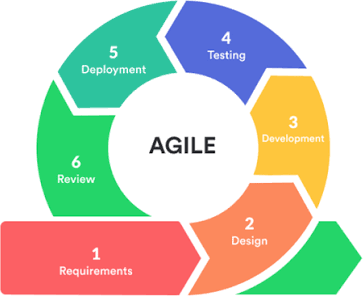
\includegraphics[width=0.50\textwidth]{images/bab5/fig2_agile.png}
    \caption{Tahapan Agile}
\end{figure}

\subsecbar{1. Requirements}
Tahap Requirements bertujuan mengidentifikasi kebutuhan sistem berdasarkan studi literatur, analisis permasalahan kesehatan mental Generasi Z, serta kebutuhan pengguna terhadap layanan pendamping kesehatan mental digital. Pada tahap ini dilakukan analisis kebutuhan fungsional dan nonfungsional sistem, penentuan fitur utama, serta penyusunan spesifikasi perangkat lunak sebagai dasar proses pengembangan.

\subsecbar{2. Design}
Tahap Design dilakukan untuk merancang solusi perangkat lunak berdasarkan kebutuhan yang telah diperoleh. Perancangan meliputi arsitektur sistem, desain basis data, desain antarmuka pengguna (\textit{User Interface}), serta perancangan arsitektur Multi-Agent Artificial Intelligence yang mengoordinasikan berbagai agen AI untuk menjalankan fungsi pendampingan kesehatan mental, analisis risiko, penyusunan diary otomatis, dan pengelolaan memori percakapan.

\subsecbar{3. Development}
Pada tahap Development, seluruh rancangan diimplementasikan menjadi perangkat lunak yang dapat dijalankan. Pengembangan dilakukan secara bertahap dengan membangun setiap modul utama LUNA, seperti \textit{Personalized Mental Health Support}, \textit{Automatic Diary}, \textit{Long-term Memory}, \textit{Mental Risk Assessment}, \textit{Early Mental Crisis Detection}, serta \textit{Voice Conversation}, kemudian mengintegrasikannya menjadi satu kesatuan sistem.

\subsecbar{4. Testing}
Tahap Testing bertujuan memastikan setiap fitur berjalan sesuai dengan kebutuhan sistem. Pengujian dilakukan terhadap fungsi-fungsi utama, integrasi antar modul, serta alur penggunaan aplikasi untuk memastikan sistem mampu memberikan layanan yang stabil, akurat, dan sesuai dengan rancangan.

\subsecbar{5. Deployment}
Tahap Deployment merupakan proses implementasi perangkat lunak sehingga dapat digunakan oleh pengguna. Pada tahap ini aplikasi dipublikasikan pada lingkungan operasional, dilakukan konfigurasi layanan pendukung, serta memastikan seluruh komponen sistem dapat beroperasi dengan baik.

\subsecbar{6. Review}
Tahap Review dilakukan sebagai proses evaluasi terhadap hasil pengembangan berdasarkan pengujian dan umpan balik pengguna. Hasil evaluasi digunakan sebagai dasar penyempurnaan fitur, peningkatan performa sistem, serta perencanaan iterasi pengembangan berikutnya sehingga LUNA dapat terus berkembang sesuai kebutuhan pengguna.
